\documentclass{article}

\usepackage[brazilian]{babel}
\usepackage{indentfirst}
\usepackage[T1]{fontenc}
\usepackage[utf8]{inputenc}
\usepackage[hidelinks]{hyperref, xurl} % \url
\usepackage{graphicx} % png

\author{Gabriel G. de Brito}
\title{Implementação simulada da arquitetura Sagui em pipeline}

\begin{document}

\maketitle

\section{Introdução}

Esse trabalho apresenta a implementação no simulador Logisim
Evolution\footnote{\url{https://github.com/logisim-evolution/logisim-evolution}}
da arquitetura Sagui em \textit{pipeline}. A implementação foi um sucesso e
todos os requisitos foram atendidos\footnote{Os requisitos foram superados,
inclusive, pois o trabalho permitia a implementação monociclo.}.

\section{O Sagui}

A figura \ref{sagui} apresenta o diagrama do processador.

\begin{figure}[ht]
	\centering
	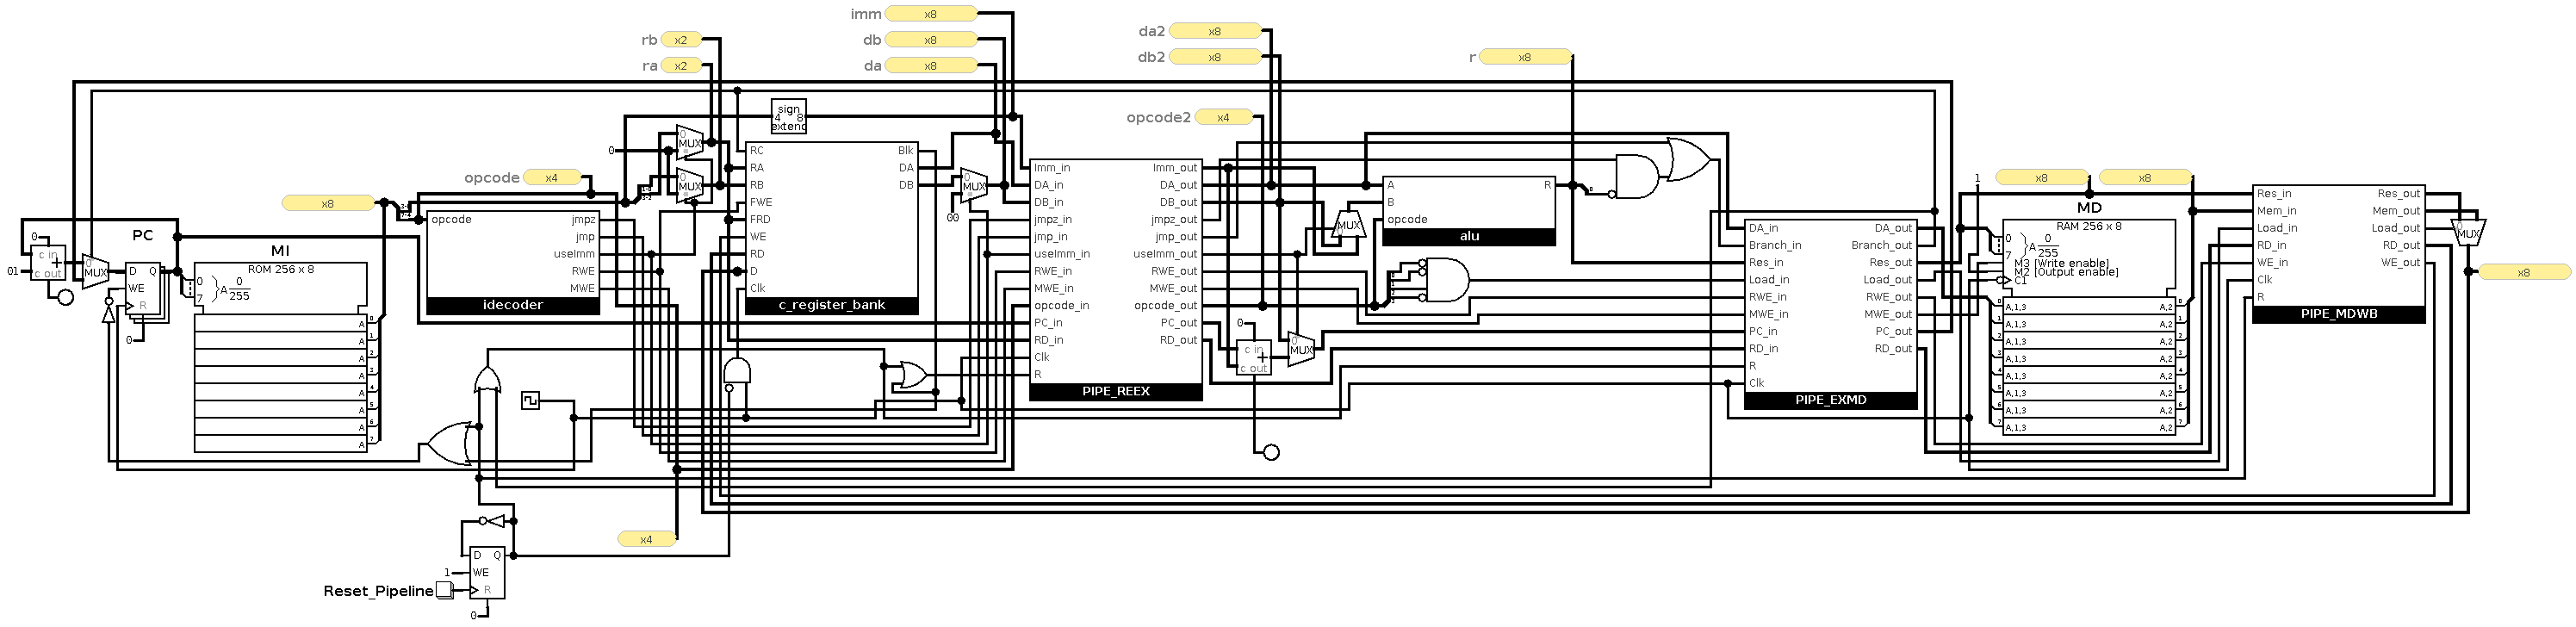
\includegraphics[width=\textwidth]{main.png}
	\caption{Diagrama do Sagui.}
	\label{sagui}
\end{figure}

O circuito principal do Sagui, além de unir os circuitos internos, realiza o
controle do \textit{pipeline} e da execução do programa, colocando uma instrução
sem efeitos colaterais quando um salto ocorre ou o banco de registradores
bloqueia a execução de uma instrução.

Os circuitos internos possuem as seguintes responsabilidades:

\begin{itemize}
	\item \textit{idecoder}: Cria sinais de controle para identificar se a
	instrução realizará um salto condicional ou incondicional, se irá utilizar
	registradores ou imediato e se escreverá no banco de registradores ou na
	memória.
	\item \textit{c\_register\_bank}: Implementa um banco de registradores com
	bloqueio de leitura.
	\item \textit{alu}: Implementa a Unidade Lógica Aritmética (ULA).
	\item \textit{PIPE\_REEX}, \textit{PIPE\_EXMD}, e \textit{PIPE\_MDWB}: separam
	os 4 estágios do \textit{pipeline}.
\end{itemize}

\section{Unidade Lógica Aritmética}

A figura \ref{ula} apresenta o diagrama da Unidade Lógica Aritmética.

\begin{figure}[ht]
	\centering
	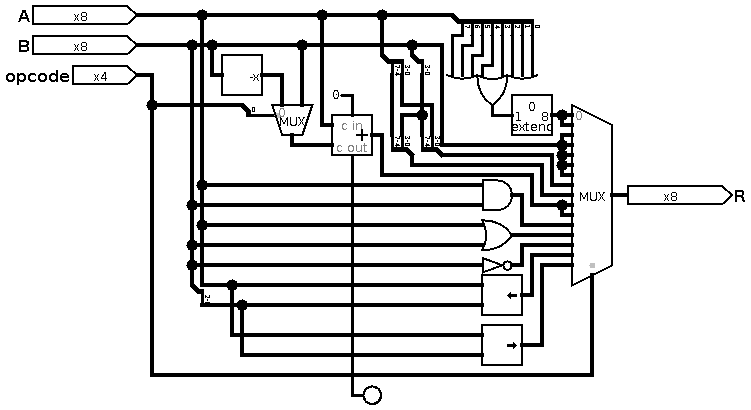
\includegraphics[width=\textwidth]{alu.png}
	\caption{Diagrama da Unidade Lógica Aritmética.}
	\label{ula}
\end{figure}

Ela seleciona a operação a ser realizada através do próprio \textit{opcode} da
instrução, pois a arquitetura possui poucas instruções e a maioria delas utiliza
o resultado da ULA. As possíveis operações são, portanto:

\begin{enumerate}
	\item \label{comp} Comparação da entrada A com 0: \textit{opcodes} 0 e 1, para
	os saltos condicionais. Propaga 1 caso A diferente de 0.
	\item Propagação da entrada B: \textit{opcodes} 2 a 6. São instruções que não
	necessitam de operações nas entradas da ULA, porém utilizam o valor de B para
	realizar saltos, mover o valor de B para outro registrador e acessar a
	memória.
	\item Concatenação da região alta de B com a baixa de A: implementa a
	instrução \textit{movh} para o \textit{opcode} 7.
	\item Concatenação da região baixa de B com a alta de A: implementa a
	instrução \textit{movl} para o \textit{opcode} 8.
	\item Soma: \textit{opcodes} 9 e 10. Realiza a soma ou a subtração, no caso em
	que multiplexadores trocam a entrada 0 do \textit{carry} do somador para 1 e a
	entrada B para o complemento do valor de B.
	\item As restantes operações são implementadas para cada um do resto dos
	\textit{opcodes}: E lógico, OU lógico, negação da comparação descrita no item
	\ref{comp}, \textit{shift} para a esquerda e \textit{shift} para a direita.
\end{enumerate}

\section{Decodificação das instruções}

O circuito \textit{idecoder} realiza a decodificação das instruções utilizando
pura lógica binária\footnote{O ato de criar e preencher uma memória de controle
é genericamente visto como mais simples que o ato de criar lógica binária para
decodificar instruções, porém o autor discorda. O primeiro ato desperta mais
preguiça nele do que o segundo.}. A figura \ref{decode} apresenta o módulo
\textit{idecoder}.

\begin{figure}[ht]
	\centering
	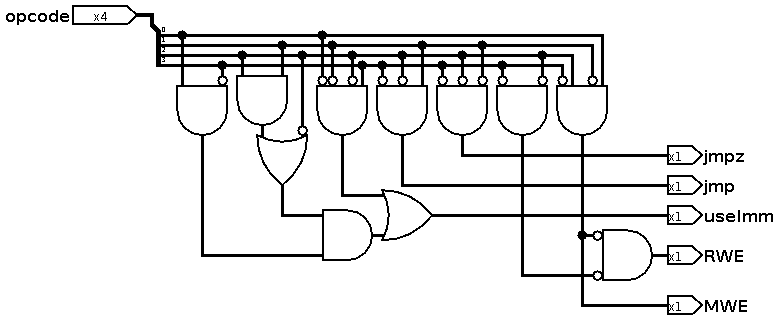
\includegraphics[width=0.5\textwidth]{idecoder.png}
	\caption{Decodificação das instruções.}
	\label{decode}
\end{figure}

\section{\textit{Pipeline}}

O \textit{pipeline} possui 4 estágios. Sendo eles:

\begin{enumerate}
	\item \textit{Fetch}, \textit{decode} e busca de dados;
	\item Execução;
	\item Acesso à memória;
	\item \textit{Write back}.
\end{enumerate}

O estado intermediário entre os estágios é salvo em módulos nomeados na forma
\textit{PIPE\_xxxx}. Um exemplo é apresentado na figura \ref{pipe}.

\begin{figure}[ht]
	\centering
	\includegraphics[width=0.5\textwidth]{pipe\_reex.png}
	\caption{Circuito intermediário ``\textit{PIPE\_REEX}'', entre os estágios 1 e
	2}.
	\label{pipe}
\end{figure}

Quando o estado precisa ser ``zerado'', ou seja, uma instrução sem efeitos
colaterais precisa ser salva, os registradores que podem causar um efeito
colateral são salvos com um valor conveniente, através de um multiplexador.

\section{Programa de teste}

Para testar a implementação, um programa em linguagem Assembly foi criado. Para
carregá-lo na máquina, gerou-se um arquivo com as instruções montadas
utilizando-se a funcionalidade de \textit{dump} do emulador
EGG\footnote{\url{https://github.com/gboncoffee/egg}}. O programa é distribuído
junto à implementação e esse documento, com o nome de "prog.txt"\footnote{A
entrega somente permitia arquivos de extensão \textit{.circ}, \textit{.txt} e
\textit{.pdf}. Portanto os \textit{.asm} e \textit{.awk} foram renomeados.}.

Como o montador do emulador utilizado não corrige as etiquetas, visto que a
maioria dos saltos precisa ser realizada a partir de registradores com
endereços, carregados via duas instruções \textit{movl} e \textit{movh}, todos
os endereços foram computados manualmente. Para facilitar a tarefa, um script em
linguagem AWK foi criado (distribuído com o nome de "addr.txt"). Qualquer
sistema UNIX com uma implementação compatível da linguagem pode executá-lo. Para
tal, usa-se a seguinte linha de comando: \verb=cat prog.txt | awk -f addr.txt=.

Para iniciar a máquina, primeiro deve-se inserir instruções sem efeito colateral
no \textit{pipeline}. Para isso, liga-se o modo "Reset Pipeline" com o botão
\textit{Reset\_pipeline} no circuito do Sagui e executa-se 1 ciclo de
\textit{clock}. Após o desligamento do modo "Reset Pipeline" a máquina estará
pronta, e os ciclos subsequentes executarão o programa da memória de instrução.

\end{document}
